\clearpage
\section{Gestione delle collection}

	\subsection{Visualizzazione dashboard} %UCU 8
	\label{visualizzazionedashboard}
			La \glossario{dashboard} (Figura \ref{fig:dashboard}) è la pagina principale dalla quale è possibile avere accesso alla lista delle \glossario{collection} presenti nel sistema e alle altre funzionalità. Per accedervi è necessario aver eseguito l'autenticazione (vedi \ref{autenticazione}). \\
			\`E possible filtrare la lista delle collection digitando il nome della collection desiderata nel campo di ricerca (1).

			\begin{figure}[H]
			\label{fig:dashboard}
				\centering 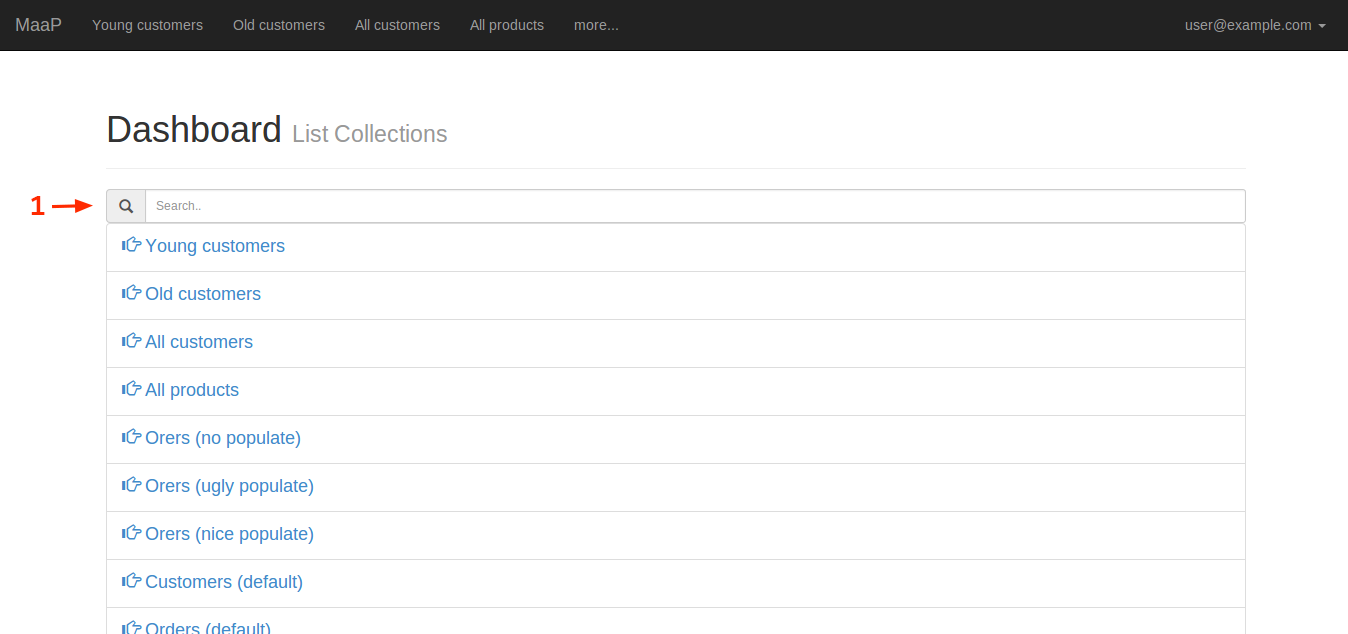
\includegraphics[width=1\textwidth]{img/dashboard.png}
			\caption{\label{fig:dashboard} Dashboard}
			\end{figure}
	
	\clearpage
	\subsection{Apertura collection index} %UCU 9
	\label{aperturacollectionindex}
		\begin{enumerate}
			\item La \glossario{collection index} è la pagina (Figura \ref{fig:collection}) in cui viene visualizzato il contenuto di una \glossario{collection} in forma tabellare. Per aprire una \glossario{collection index} (Figura \ref{fig:aperturaCollection}) è necessario cliccare sul relativo link presente nella barra dei menù (1) oppure nel link visualizzato nella pagina \glossario{dashboard} (2).

			\begin{figure}[H]
				\centering 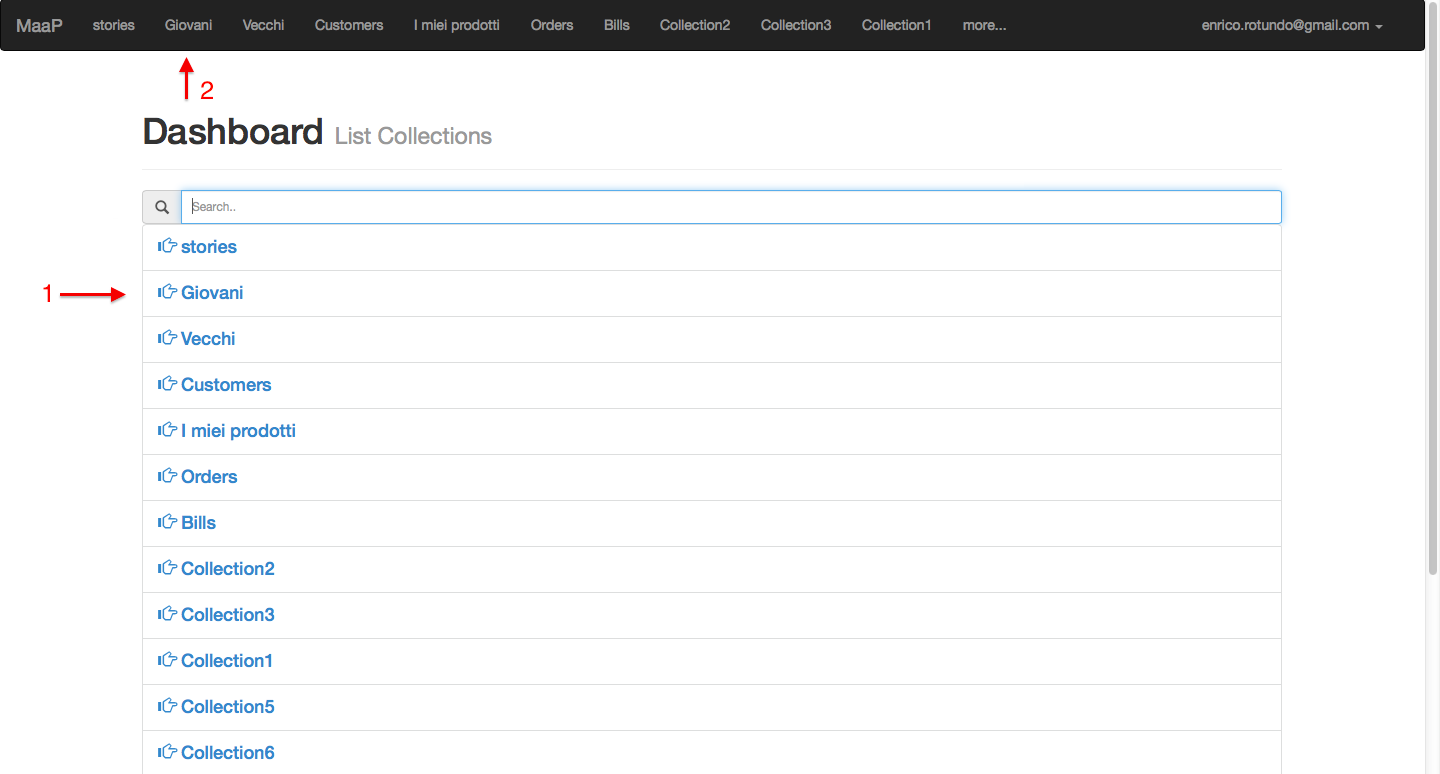
\includegraphics[width=1\textwidth]{img/aperturaCollection.png}
			\caption{ \label{fig:aperturaCollection} Index di una collection}
			\end{figure}


			\item La pagina \glossario{collection index} (Figura \ref{fig:collection}) visualizzerà l'intero contenuto della \glossario{collection}. La tabella visualizza i documenti dei quali è possibile aprire la \glossario{showpage} (vedi \ref{aperturashowpage}) cliccando sul relativo link (1).

			\begin{figure}[H]
				\centering 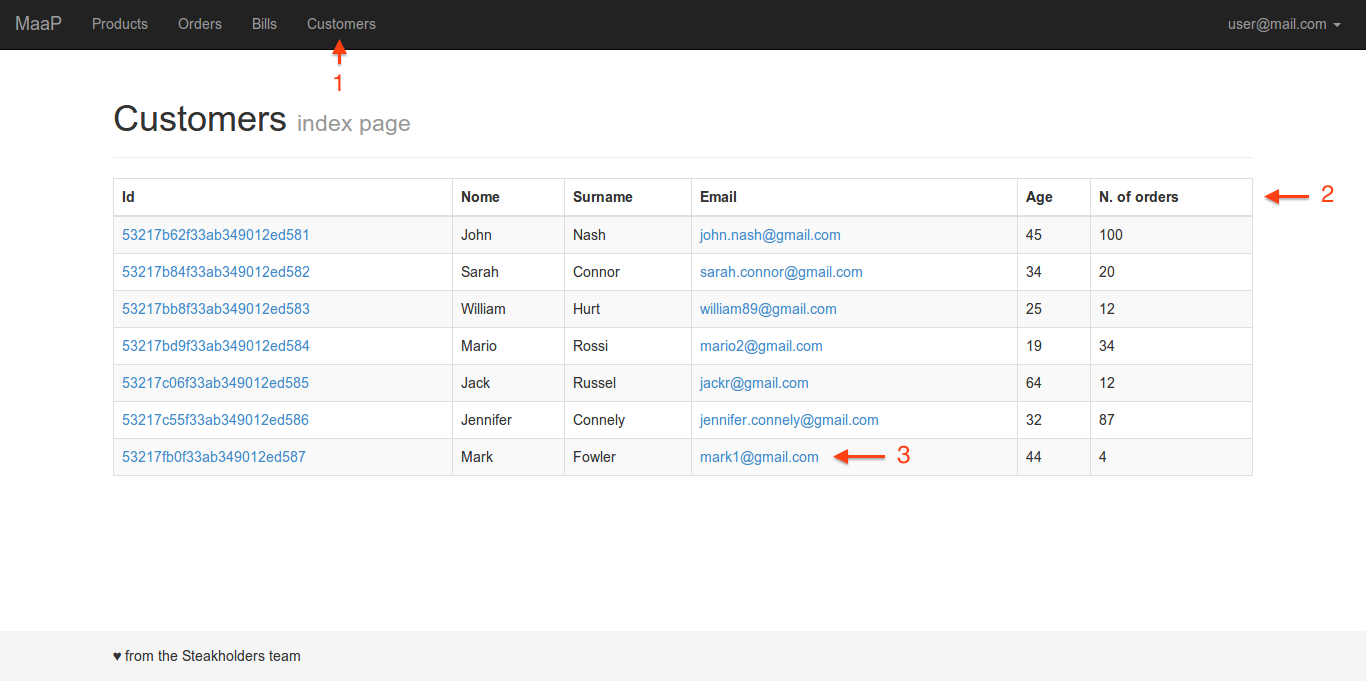
\includegraphics[width=1\textwidth]{img/collection.png}
			\caption{ \label{fig:collection} Index di una collection}
			\end{figure}
		\end{enumerate}

	\clearpage
	\subsection{Apertura della show-page di un document} %UCU 9.
	\label{aperturashowpage}
		\begin{enumerate}
			\item La \glossario{showpage} di un \glossario{document} visualizza gli attributi del documento in forma tabellare (Figura \ref{fig:showpage}). Per accedere ad una show page è necessario posizionarsi nella \glossario{collection index} di appartenenza (vedi \ref{aperturacollectionindex}) e seguire il punto (1).

			\begin{figure}[H]
			\label{fig:showpage}
				\centering 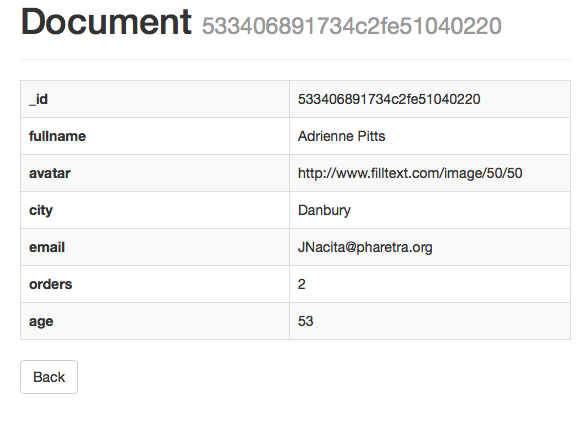
\includegraphics[width=0.7\textwidth]{img/showpage.png}
			\caption{\label{fig:showpage} Show page di un documento}
			\end{figure}
		\end{enumerate}

	% \clearpage
	\subsection{Visualizzazione show-page attributi innestati} % 9.1.1
			La presenza di \glossario{document} innestati (Figura \ref{fig:attributiInnestati}) viene evidenziata dalla visualizzazione dell'attributo come un link (1), attraverso il quale è possibile accedere alla show page. Nell esempio riportato in Figura \ref{fig:attributiInnestati} i punti (2) e (3) evidenziano come sia possibile avere molteplici attributi innestati e quindi visualizzabili.

			\begin{figure}[H]
			\label{fig:showpage}
				\centering 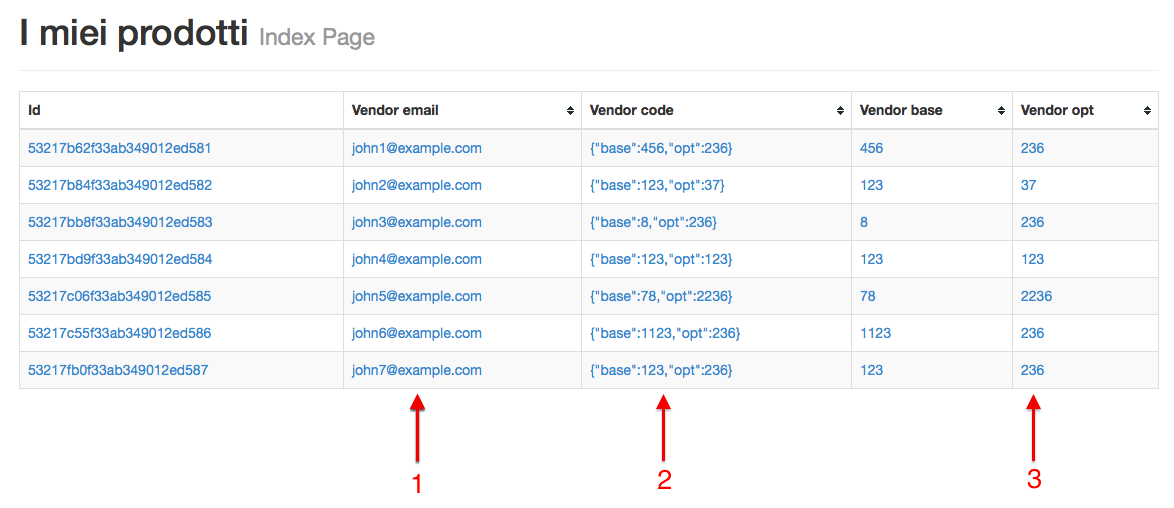
\includegraphics[width=0.7\textwidth]{img/attributiInnestati.png}
			\caption{\label{fig:attributiInnestati} Esempio di attributo innestato}
			\end{figure}


			%\subsection{Filtra risultati} %TODO viene implementato in RA  attributiInnestati
